\documentclass[12pt,fleqn]{article}\usepackage{../common}
\begin{document}
Ders 11

Onceki derste cok degiskenli fonksiyonlari min, maks uzerinden
inceledik. Bu derste bu tur fonksiyonlarin herhangi bir yondeki
varyasyonunu nasil hesaplayacagimizi gorecegiz. Bunu yapabilmek icin daha
fazla kavramsal araclara ihtiyacimiz var. 

Bugunku konumuz diferansiyeller. 

Diferansiyeller

Tek degiskenli Calculus'tan dolayli (implicit) diferansiyel almayi
biliyoruz herhalde. Mesela elimizde

\[ y = f(x) \]

var. Dolayli turevler ile $x$ uzerindeki sonsuz kucuk bir degisimi $y$
uzerindeki sonsuz kucuk bir degisime baglayabiliyoruz. 

\[ dy = f'(x) dx \]

Ornek

\[ y = sin^{-1}(x) \]

Bu formulun turevini bulmak icin, soyle bir zincir takip
edebiliriz. Usttekine tersten bakalim

\[ x = sin(y) \]

O zaman

\[ dx = cos(y)dy \]

\[ 
\frac{dy}{dx} = \frac{1}{cos(y)} = \frac{1}{\sqrt{1-x^2}}
 \]

Esitligin sag tarafini nasil elde ettik? Hatirlayalim

\[ cos^2(y) + sin^2(y) = 1 \]

\[ cos (y) = \sqrt{1 - sin^2y} \]

$sin^2(y)$ nedir? 

\[ y = sin^{-1}(x) \]

\[ sin(y) = sin(sin^{-1}(x)) \]

Ters sinus fonksiyonunun sinusu alinirsa, geriye sadece $x$ kalir. 

\[ sin(y) = x \]

O zaman

\[ cos (y) = \sqrt{1 - x^2} \]

Iste bu tur $dy,dx$ iceren formulleri kullanacagiz, bu derste cok
degiskenli ortamda bunu yapacagiz. 

Tam Diferansiyeller

Eger $f(x,y,z)$ varsa, 

\[ df = f_xdx + f_ydy + f_zdz \]

Diger notasyonla

\[ df = \frac{\partial f}{\partial x}dx + \frac{\partial f}{\partial y}dy + 
\frac{\partial f}{\partial z}dz \]

Bu formulun hesapladigi nedir? Elde edilen bir sayi, matris, vektor
degildir. Bu degisik turden bir nesne ve bu nesneleri manipule etmenin,
kullanmanin kendine has kurallari var. Onlari nasil kullanacagimizi
ogrenmemiz gerekiyor. 

Onlari nasil irdelemek gerekir? Bunu cevaplayabilmek icin onlari nasil
``gor\textbf{me}memiz'' gerektigini anlamamiz lazim. 

Onemli

$df$ ile $\Delta f$ farkli seylerdir.

Bir kere $\Delta f$ bir sayidir, onu hesaplamak icin $\Delta x, \Delta y,
\Delta z$, vs.. gibi 
sayilar kullaniriz. Kiyasla $df$ bir sayi degildir, onu gostermenin 
tek yolu diger diferansiyeller uzerindendir. 

Diferansiyelleri, yani $dx, dz$ gibi nesneleri bir ``yerine baska seyler
koyabileceginiz bir tur isaret (placeholder)'' gibi
dusunebilirsiniz. Onlarin sonsuz kucuklukteki degisimi temsil ettigi de
dogrudur, ama hoca bu tanimi pek sevmiyor. Bu ``isaretleyici'' nesnelere
degisim degerlerini (evet, sayisal olarak, ama yaklasiksal baglamda) verirsek,
esitligin sol tarafinda $df$ icin bir teget duzlem yaklasiksallamasi elde
edebiliriz. 

O zaman diferansiyeller 

1) $x,y,z$'deki degisimin $f$'i nasil etkilediginin kodlarini / sifrelerini
(encode) icerirler. Tam diferansiyel formulu hakkinda soyleyebilecegimiz en
genel soz budur.

2) Onlar $\Delta x, \Delta
y, \Delta z$ gibi varyasyonlar icin bir isaret / yer tutucu 
gorevi gorurler ve onlarin sayesinde $\Delta f \approx f_x\Delta x + f_y \Delta y + f_z
\Delta z$ 
yaklasiksal formulunu elde etmek mumkun olur. $\Delta f$ formulu ile $df$ 
formulunde birincinin $\approx$ ikincisinin $=$ kullandigina dikkatinizi cekerim.

3) Tam diferansiyel uzerinde yapabilecegimiz bir diger islem, tum formulu
herkesin bagli oldugu bir baska degiskene bolmektir. Diyelim ki $x,y,z$
degiskenlerinin hepsi de $t$ adindaki bir baska degiskene bagli. O zaman
tum formulu $dt$'ye bolerek $t$ bazindaki degisimin $f$'i nasil
etkiledigini gorebilirim, yani $df/dt$'yi hesaplayabilirim. Yani sunu elde
ederim, 

\[ \frac{df}{dt} = f_x\frac{dx}{dt} + f_y\frac{dy}{dt} + f_z\frac{dz}{dt} \]

ki bu $x=x(t),y=y(t),z=z(t)$ ise olabilir. Boylece $f$'in degisim oranini
(rate of change) elde ederim. 

Bu arada ustteki formul Zincirleme Kanunu (Chain Rule) olarak ta bilinir,
cunku $x,y,z$ degiskenleri $t$'ye bagli, ve ustteki formulle ``zincirleme
olarak'' $f$'den $x,y,z$, oradan $t$'ye gidiyoruz, ve degisim orani
hesabini elde ediyoruz.

Ustteki 2. ifade niye gecerlidir? Matematiksel olarak onu nasil
hesaplayabilirim? 

1. Deneme

\[ df = f_xdx + f_ydy + f_zdz \]

ile baslariz. Eger $x=x(t)$ ise, o zaman

\[ dx = x'(t)dt \]

ifadesi de dogrudur. Ayni sekilde

\[ dy = y'(t)dt \]

\[ dz = z'(t)dt \]

Bunlari ana formulde yerine koyarsak

\[ df = f_xx'(t)dx + f_yy'(t)dy + f_zz'(t)dz \]

olur. Tum formulu $dt$'ye bolersem, Zincirleme Kanununu elde ederim. 

Bu isliyor, fakat diyelim ki cok suphecisiniz, ve diferansiyel kavramina
hala inanmiyorsunuz. Bu ispatta mesela $dx = x'(t)dt$ gibi yine
diferansiyel alma islemini kullandim. Aslinda Zincirleme Kanunu boyle
ispatlanmiyor. 

2. Deneme

Simdiye kadar guvendigimiz kavramlardan biri yaklasiksallama
formulumuz. Ona guveniyoruz. O da diyor ki 

\[ \Delta f \approx f_x\Delta x + f_y \Delta y + f_z \Delta z \]

Her seyi $\Delta t$ ile bolelim. 

\[ \frac{\Delta f}{\Delta t} \approx 
\frac{f_x\Delta x + f_y \Delta y + f_z \Delta z }{\Delta t}\]

Burada sayilar kullaniyorum, $\Delta ..$ ile ifade edilenler sayidir. Bir
``difereansiyele'' bolmek ne demektir bilmiyoruz, ama bir sayiyla bolmenin
ne demek oldugunu iyi biliyoruz. 

Sunu da biliyoruz - eger $\Delta t \to 0$ ise 

\[ \frac{\Delta f}{\Delta t} \to \frac{df}{dt} \]

Turevlerin tanimi matematiksel olarak budur. Bu durum tum degiskenler icin
de gecerlidir. Mesela

\[ \frac{\Delta x}{\Delta t} \to \frac{dx}{dt} \]

O zaman bolumun tamami, $\Delta t \to 0$ iken alttaki gibi olur,
yaklasiksallik $\Delta t$ sifira dogru yaklasikca esitlige donusur.

\[ \frac{df}{dt} = f_x\frac{dx}{dt} + f_y\frac{dy}{dt} + f_z\frac{dz}{dt} \]

Ornek

\[ w = x^2y + z \]

\[ x = t \]

\[ y = e^t \]

\[ z = sin(t) \]

\[ \frac{dw}{dt} = 2xy \frac{dx}{dt} + x^2 \frac{dy}{dt} + 1 \frac{dz}{dt}\]

\[ = 2te^t 1 + t^2e^t+cos(t) \]

\[ = 2te^t + t^2e^t+cos(t) \]

Bu sonuca baska turlu nasil erisebilirdik? 

Ana formul $w$ icine tum degiskenlerin $t$ bazinda karsilikarini gecirelim

\[ w(t) = t^2e^t + sin(t) \]

O zaman

\[ \frac{dw}{dt} = 2te^t + t^2e^t + cos(t) \]

Uygulama

Calculus'taki Turevlerde Carpim (Product Rule) ve Bolum Kanunlarini
(Quotient Rule) dogrula.

\[ f = uv \]

\[ u=u(t) \]

\[ v=v(t) \]

Tam Diferansiyeli uygulayalim

\[ \frac{d(uv)}{dt} = f_u\frac{du}{dt} + f_v \frac{dv}{dt}\]

\[  = v\frac{du}{dt} + u \frac{dv}{dt}\]

Boylece Carpim Kanununu aynen elde etmis olduk. 

Bolum Kanunu icin

\[ g = \frac{u}{v} \]

\[ u=u(t) \]

\[ v=v(t) \]

\[ \frac{d(u/v)}{dt} = \frac{1}{v} \frac{du}{dt} + \frac{-u}{v^2}\frac{dv}{dt}\]

Tekrar duzenlersek

\[ = \frac{u'v - v'u}{v^2} \]

Bolum Kanununu elde ettik.

Simdi biraz daha cilginca bir sey yapalim. Iddia ediyorum ki daha fazla
degisken icin Zincirleme Kanununu kullanabilirim. 

\[ w = f(x,y), \ x = x(u,v), \ y = y(u,v) \]

Bu degisken isimleri belki acaip, anlamsiz geliyor, ama daha somut bir
ornek olarak sunu dusunelim. Mesela kutupsal kordinat sistemine gidip
gelmem gerekiyor ve $x,y$'nin bagimli oldugu degiskenler $r$ ve
$\theta$. Belki de turevlerin kutupsal forma nasil yansidigina gormek
istiyorum, gibi..

Devam edelim. Turev almak icin bir yontem, $x,y$'yi yerlerine koymak ve

\[ w = f(x(u,v),y(u,v)) \]

hesabi yapmak. Boylece $w$ formulu $u,v$ bazinda bir formul haline
gelir. Sonra kismi turevleri alirim, vs. Ama bu cok cetrefil bir islem
olabilir. Alternatif?

$\partial w/\partial u$, $\partial w/\partial v$ kismi turevlerini $\partial w/\partial x$ ve $\partial w/\partial y$ bazinda goster.

Ayrica $x_u, x_w, y_u, y_v$'yi goster. 

\[ dw =  f_xdx + f_y dy\]

Biz $dx$ ve $dy$'den kurtulmak istiyoruz cunku cevap istedigimiz sorulardan
biri ``$u,v$ biraz degisince $w$ ne kadar degisir'' seklindeki
sorular. Devam edelim

\[ = f_x \bigg( x_u du + x_y dv \bigg) + 
f_y \bigg( y_u du + y_v dv \bigg) \]

Yani $dx$ ve $dy$'yi, tekrar tam diferansiyel kuralini kullanarak actim. 

\[ = \bigg(f_x x_u + f_yy_u \bigg)du  + 
\bigg(f_xx_u + f_yy_v \bigg) dv \]

Bu formulde kismi turevler soyle gosterilebilir

\[ = 
\underbrace{(f_x x_u + f_yy_u )}_{\partial f/\partial u}du  + 
\underbrace{(f_xx_u + f_yy_v)}_{\partial f/\partial v}dv
\]

Yani

\[ \frac{\partial f}{\partial u} = 
\frac{\partial f}{\partial x}\frac{\partial x}{\partial u} +
\frac{\partial f}{\partial y}\frac{\partial y}{\partial u} 
\]

\[ \frac{\partial f}{\partial v} = 
\frac{\partial f}{\partial x}\frac{\partial x}{\partial v} +
\frac{\partial f}{\partial y}\frac{\partial y}{\partial v} 
\]

Ustteki sonuca vardik cunku, mesela $\partial f/\partial u$'nun olmasi gereken yer belli, 
hemen $du$'dan once gelmeli.

Not: Ustteki iki formulde, mesela birincisinde, insanin icinden hem bolum,
hem bolende olan $\partial x$ ve $\partial y$'leri iptal etmek
gelebilir. Ama bunu yaparsak

\[ \frac{\partial f}{\partial u} = 
\frac{\partial f}{\partial u} + \frac{\partial f}{\partial u} 
\]

gibi bir formul cikardi, ki bu formul dogru olmazdi. Cunku bu tur bir iptal
operasyonu yanlistir, bunlar kismi turevler, tam turevler (total
derivatives) degil. Zaten $d$ yerine kivrik d, yani $\partial$ sembolu
kullanmamizin sebebi de bu -- bize hatirlatici olmalari icin. $d$'ler ile
yapabilecegimiz bazi basitlestirme islemlerini $\partial$'lar ile
yapamadigimizi hatirlamak amaciyla degisik semboller kullaniyoruz. 

Ornek

Kutupsal kordinatlarimiz varsa, degisim formulu soyledir

\[ x = r cos(\theta) \]

\[ y = r sin(\theta) \]

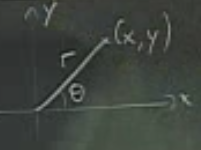
\includegraphics[height=3cm]{11_1.png}

Ve elimizde bir $f=f(x,y)$ var ise, ustteki $x,y$ formullerini yerine
koyup $f$ formulunu $r,\theta$ bazinda elde edebiliriz.

Sonra su hesabi yapariz

\[ \frac{\partial f}{\partial r} = 
\frac{\partial f}{\partial x}
\frac{\partial x}{\partial r} +
\frac{\partial f}{\partial y}
\frac{\partial y}{\partial r}
 \]

\[ = f_xcos(\theta) + f_y sin(\theta) \]

Bu tur numaralar sonraki derste faydali olacak. Mesela gradyan vektoru
kismi turevlerden olusan bir vektordur. 

\[ \nabla f = <f_x,f_y,f_x> \]

Yani aslinda bir diferansiyeli kismi turevleri bir paket halinde bir araya
getirip size sunan bir sey olarak gorebilirsiniz. Gradyan vektor de bu
paketlemeyi degisik bir sekilde yapan bir diger nesnedir. 


\end{document}
